% ============================================================
% 第9章：数列的概念——从离散到无限
% ============================================================

\chapter{数列的概念——从离散到无限}

\begin{applicationbox}
\textbf{学完本章你能做什么？}
\begin{enumerate}
  \item 理解\textbf{数列}是什么——按顺序排列的一列数，是离散版本的函数
  \item 掌握\textbf{等差数列}和\textbf{等比数列}的通项与求和
  \item 学会用\textbf{递推公式}表示数列，并推导通项
  \item 判断数列的\textbf{单调性}和\textbf{有界性}——为极限学习做准备
\end{enumerate}
\end{applicationbox}


% ============================================================
\section{从函数到数列——连续 vs 离散}
% ============================================================

前8章我们学的函数，自变量 \(x\) 可以在实数范围内连续变化（取任意值）。

但现实中有很多情况，自变量只能取\textbf{正整数}：

\begin{itemize}
  \item 第1天存 100 元，第2天存 200 元，第3天存 300 元……
  \item 第1代细菌有 1 个，第2代有 2 个，第3代有 4 个……
  \item 第1个月还款 5000 元，第2个月还款 4980 元，第3个月还款 4960 元……
\end{itemize}

这些按\textbf{顺序排列}的一列数，就叫\textbf{数列}。

\begin{center}
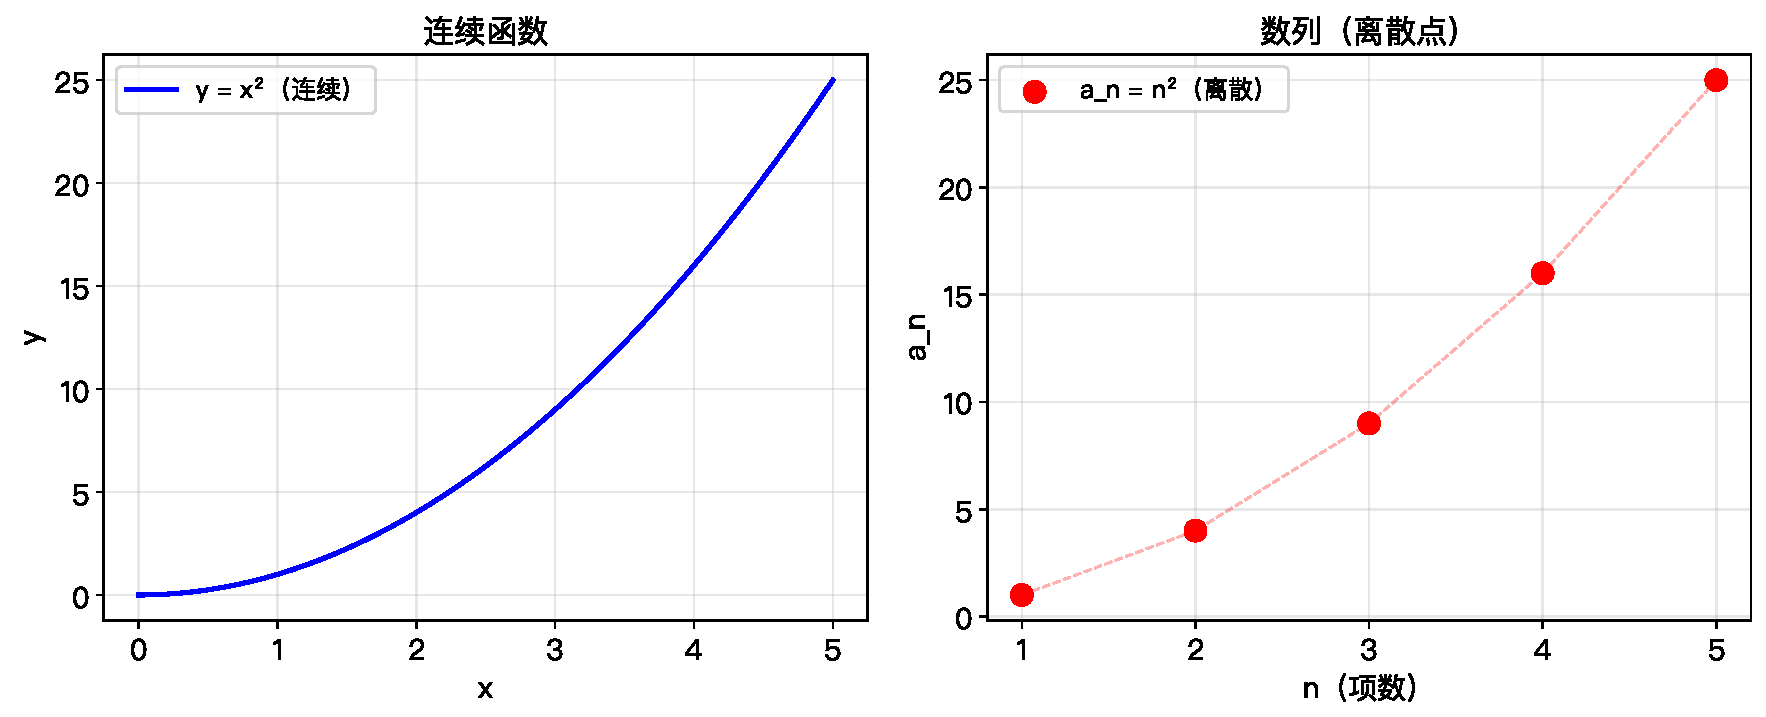
\includegraphics[width=0.8\textwidth]{figures/ch09_continuous_vs_discrete.pdf}
\end{center}

左边是连续函数 \(y = x^2\)，右边是离散数列 \(a_n = n^2\)——同样的公式，但数列只取正整数点。


% ============================================================
\section{数列的定义}
% ============================================================

\begin{definitionbox}[数列]
按一定顺序排列的一列数称为\textbf{数列}（读作 shù liè，英文 sequence）。

记作：
\[
a_1, a_2, a_3, \ldots, a_n, \ldots
\]

其中：
\begin{itemize}
  \item \(a_1\) 是\textbf{第1项}（首项），\(a_n\) 是\textbf{第 \(n\) 项}（通项）
  \item \(n\) 是\textbf{项数}（下标，正整数）
  \item 整个数列简记为 \(\{a_n\}\) 或 \(a_n\)（习惯上混用）
\end{itemize}

\textbf{数列和函数的关系：}
\[
\text{数列 } a_n = f(n) \quad (n = 1, 2, 3, \ldots)
\]
数列就是以\textbf{正整数}为定义域的函数。
\end{definitionbox}

\begin{examplebox}[1——写出数列的前几项]
写出 \(a_n = 2n - 1\) 的前 5 项：

\[
n=1: a_1 = 1,\; n=2: a_2 = 3,\; n=3: a_3 = 5,\; n=4: a_4 = 7,\; n=5: a_5 = 9
\]

所以数列为：\(1, 3, 5, 7, 9, \ldots\)（奇数数列）
\end{examplebox}


% ============================================================
\section{等差数列——均匀变化}
% ============================================================

\begin{definitionbox}[等差数列]
如果数列从第2项起，每一项与前一项的差等于同一个常数，则称该数列为\textbf{等差数列}（读作 děng chā shù liè）。

\[
a_{n+1} - a_n = d \quad (\text{\(d\) 是常数，叫\textbf{公差}})
\]

\textbf{通项公式：}
\[
a_n = a_1 + (n-1)d
\]

\textbf{前 \(n\) 项和：}
\[
S_n = \frac{n(a_1 + a_n)}{2} = na_1 + \frac{n(n-1)}{2}d
\]
\end{definitionbox}

\begin{examplebox}[2——等差数列]
已知等差数列首项 \(a_1 = 3\)，公差 \(d = 2\)。

数列：\(3, 5, 7, 9, 11, \ldots\)

通项：\(a_n = 3 + (n-1) \times 2 = 2n + 1\)

前 5 项和：
\[
S_5 = \frac{5(3 + 11)}{2} = \frac{5 \times 14}{2} = 35
\]

验证：\(3 + 5 + 7 + 9 + 11 = 35\) [OK]
\end{examplebox}

\begin{examplebox}[3——等差数列的应用]
小明第一天背 10 个单词，之后每天比前一天多背 3 个。第 30 天背多少个？

解：\(a_1 = 10\)，\(d = 3\)，\(n = 30\)
\[
a_{30} = 10 + (30-1) \times 3 = 10 + 87 = 97
\]

30 天共背了多少个？
\[
S_{30} = \frac{30(10 + 97)}{2} = 15 \times 107 = 1605
\]
\end{examplebox}


% ============================================================
\section{等比数列——成倍变化}
% ============================================================

\begin{definitionbox}[等比数列]
如果数列从第2项起，每一项与前一项的比等于同一个常数，则称该数列为\textbf{等比数列}（读作 děng bǐ shù liè）。

\[
\frac{a_{n+1}}{a_n} = q \quad (\text{\(q\) 是常数，叫\textbf{公比}，\(q \neq 0\)})
\]

\textbf{通项公式：}
\[
a_n = a_1 q^{n-1}
\]

\textbf{前 \(n\) 项和（\(q \neq 1\)）：}
\[
S_n = a_1 \frac{1 - q^n}{1 - q}
\]
\end{definitionbox}

\begin{examplebox}[4——等比数列 vs 等差数列]
\begin{center}
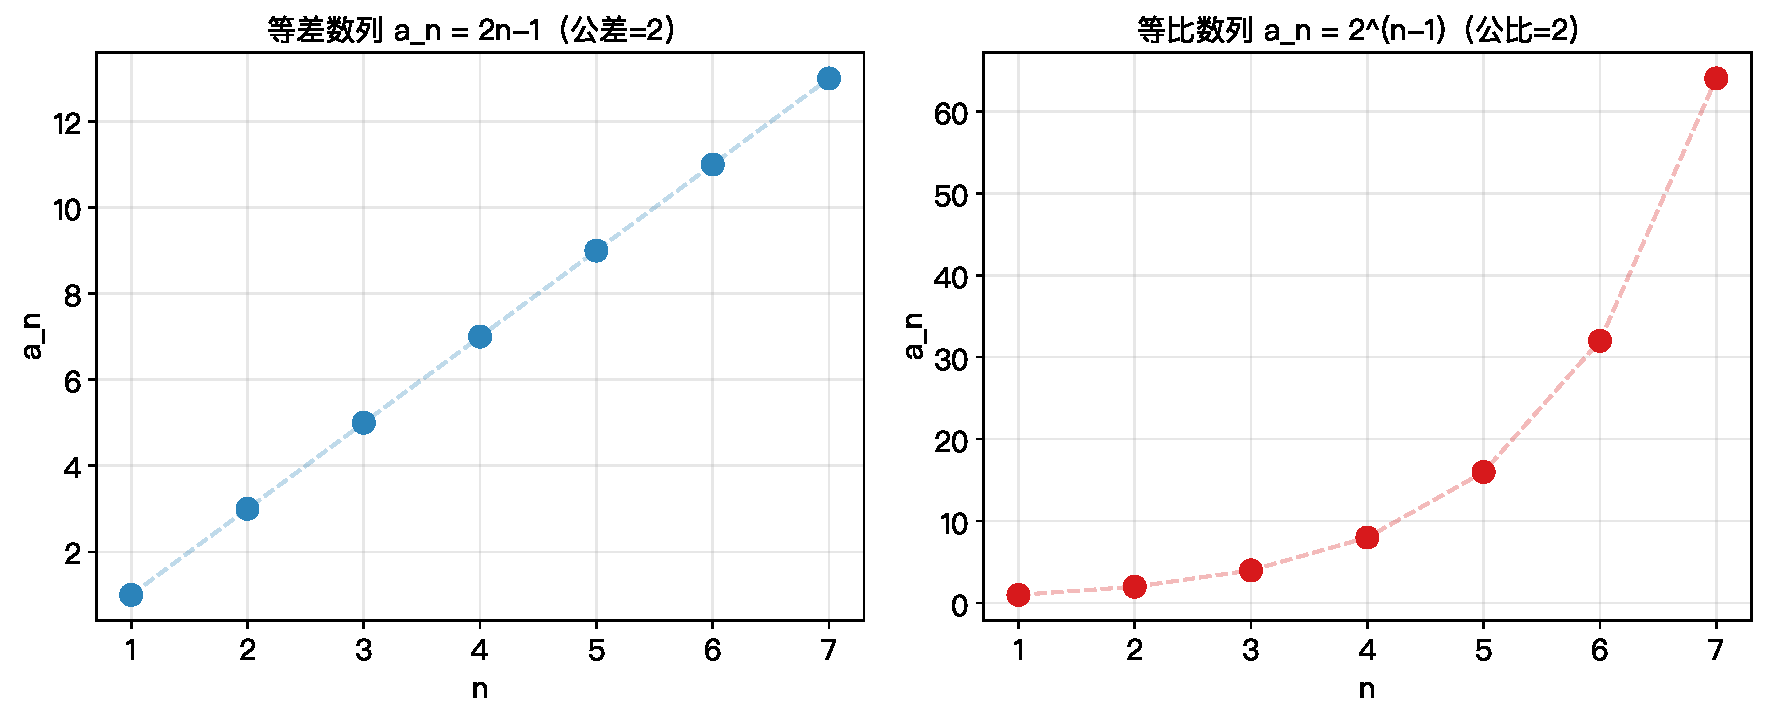
\includegraphics[width=0.85\textwidth]{figures/ch09_arithmetic_geometric.pdf}
\end{center}

\textbf{左图：}等差数列 \(a_n = 2n-1\)——增长是\textbf{均匀}的（每天+2）。\\
\textbf{右图：}等比数列 \(a_n = 2^{n-1}\)——增长越来越\textbf{快}（每天$\times$2）。

\textbf{关键区别：}等差是线性增长，等比是指数增长。
\end{examplebox}

\begin{examplebox}[5——等比数列的应用]
某种细菌每 1 小时分裂一次（数量翻倍）。初始 100 个，8 小时后有多少个？

解：\(a_1 = 100\)，\(q = 2\)，\(n = 8\)
\[
a_8 = 100 \times 2^{8-1} = 100 \times 2^7 = 100 \times 128 = 12800
\]

8 小时内总共产生了多少个（含初始）？
\[
S_8 = 100 \times \frac{1 - 2^8}{1 - 2} = 100 \times \frac{1 - 256}{-1} = 100 \times 255 = 25500
\]
\end{examplebox}


% ============================================================
\section{递推公式——用前一项定义后一项}
% ============================================================

有时候数列没有明确的通项公式，而是通过\textbf{递推关系}定义。

\begin{definitionbox}[递推公式]
如果数列的每一项由前一项（或前几项）通过一个公式确定，这个公式叫\textbf{递推公式}。

常见形式：
\[
a_{n+1} = f(a_n) \quad \text{或} \quad a_{n+1} = p a_n + q
\]
\end{definitionbox}

\begin{examplebox}[6——由递推求通项]
已知 \(a_1 = 1\)，\(a_{n+1} = 2a_n + 1\)，求 \(a_5\)。

\textbf{逐项计算：}
\[
a_1 = 1
\]
\[
a_2 = 2 \times 1 + 1 = 3
\]
\[
a_3 = 2 \times 3 + 1 = 7
\]
\[
a_4 = 2 \times 7 + 1 = 15
\]
\[
a_5 = 2 \times 15 + 1 = 31
\]

数列：\(1, 3, 7, 15, 31, \ldots\)

\textbf{猜想通项：} \(a_n = 2^n - 1\)（验证：\(2^1-1=1\)，\(2^2-1=3\)，\(2^3-1=7\) [OK]）
\end{examplebox}


% ============================================================
\section{数列的单调性与有界性}
% ============================================================

和函数一样，数列也有单调性和有界性——这对后续学习极限至关重要。

\begin{definitionbox}[数列的单调性与有界性]
\textbf{单调递增：} \(a_{n+1} \ge a_n\) 对所有 \(n\) 成立。\\
\textbf{单调递减：} \(a_{n+1} \le a_n\) 对所有 \(n\) 成立。\\
\textbf{有上界：}存在 \(M\) 使得 \(a_n \le M\) 对所有 \(n\) 成立。\\
\textbf{有下界：}存在 \(m\) 使得 \(a_n \ge m\) 对所有 \(n\) 成立。
\end{definitionbox}

\begin{examplebox}[7——单调有界数列]
数列 \(a_n = 1 - \dfrac{1}{n}\)：

\begin{center}
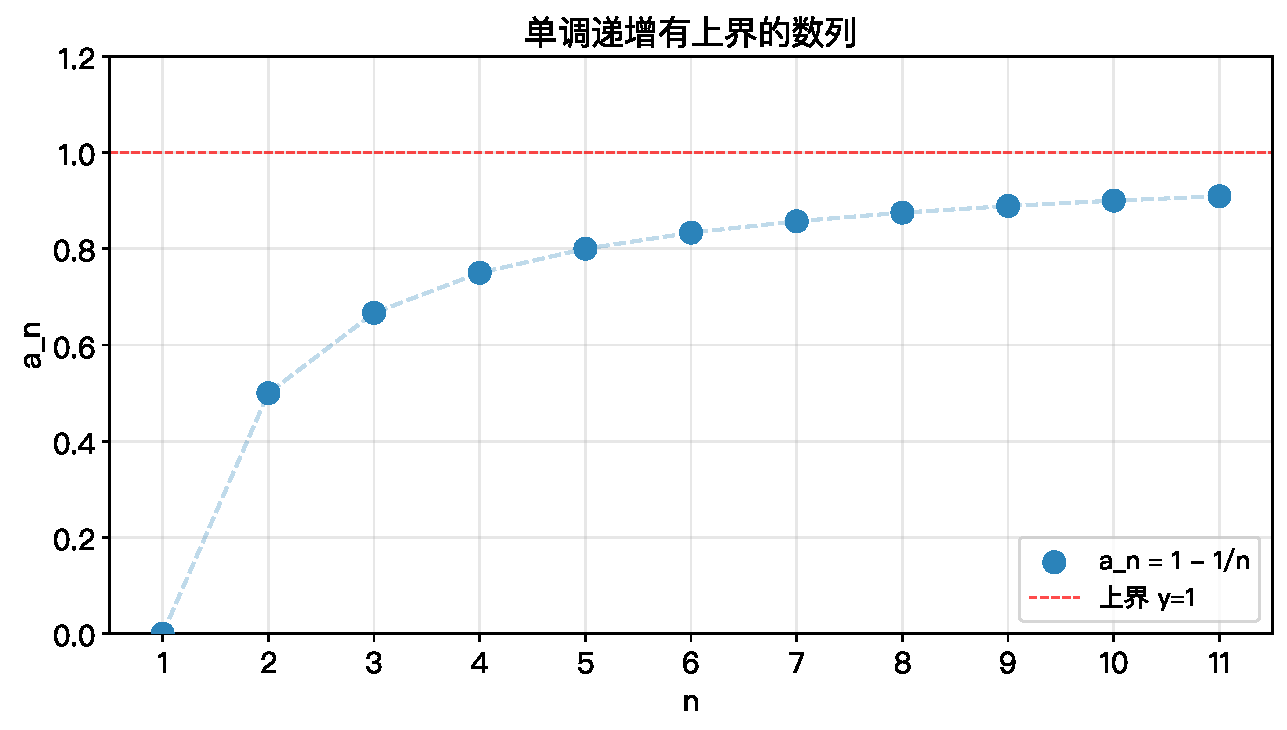
\includegraphics[width=0.75\textwidth]{figures/ch09_monotonic_bounded.pdf}
\end{center}

\textbf{单调性：} \(a_n = 1 - \frac{1}{n}\)，当 \(n\) 增大时 \(\frac{1}{n}\) 减小，所以 \(a_n\) 增大 \(\rightarrow\) \textbf{单调递增}。

\textbf{有界性：} \(a_n < 1\) 对所有 \(n\) 成立（因为 \(\frac{1}{n} > 0\)），所以 1 是\textbf{上界}。\\
同时 \(a_n \ge a_1 = 0\)，0 是\textbf{下界}。\\
\(\rightarrow\) 单调递增有上界（且下界）。
\end{examplebox}

\begin{examplebox}[8——摆动数列]
数列 \(a_n = \dfrac{(-1)^n}{n}\)：

\begin{center}
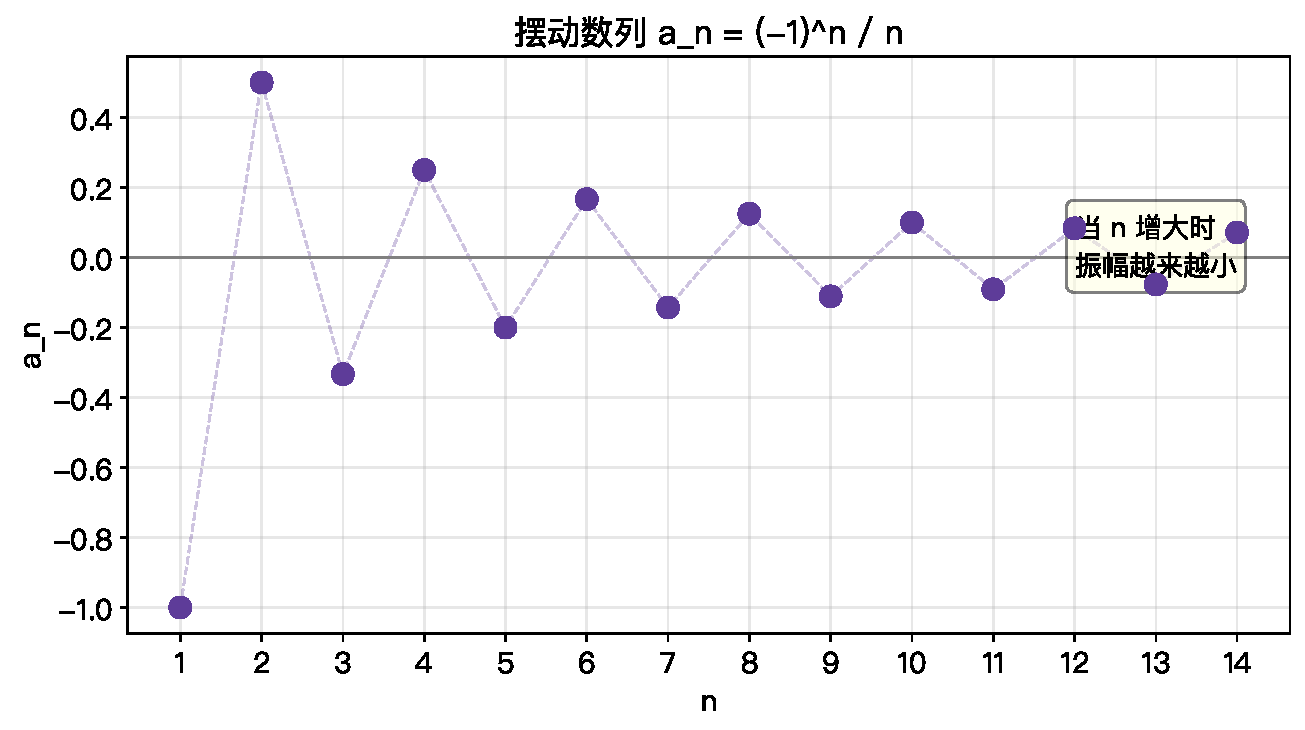
\includegraphics[width=0.75\textwidth]{figures/ch09_oscillating.pdf}
\end{center}

这个数列在正负之间摆动，但\textbf{振幅越来越小}，趋近于 0。\\
它\textbf{不是单调的}，但\textbf{是有界的}（\(-1 \le a_n \le 1\)）。
\end{examplebox}


% ============================================================
\section{符号卡片}
% ============================================================

\begin{symbolcard}
\(\{a_n\}\) & \verb|{a_n}| & 读作"数列 a n" & 数列 \(a_1, a_2, a_3, \ldots\) \\
\(d\) & —— & 读作"公差" & 等差数列中相邻项的差 \\
\(q\) & —— & 读作"公比" & 等比数列中相邻项的比 \\
\(S_n\) & \verb|S_n| & 读作"S n" & 前 \(n\) 项和 \\
\(a_{n+1} = f(a_n)\) & —— & —— & 递推公式 \\
\end{symbolcard}


% ============================================================
\section{代码验证}
% ============================================================

\begin{lstlisting}[caption=数列的数值验证]
import numpy as np

# 1. 等差数列
print("=== 等差数列 a_n = 2n+1 ===")
a1, d = 3, 2
for n in range(1, 9):
    an = a1 + (n-1)*d
    print(f"  a_{n} = {an}", end="")
print()

# 前n项和
S5 = 5*(a1 + (a1+4*d)) // 2
print(f"  S_5 = {S5}")

print()

# 2. 等比数列
print("=== 等比数列 a_n = 2^(n-1) ===")
for n in range(1, 11):
    an = 2**(n-1)
    print(f"  a_{n:2d} = {an:4d}", end="")
print()

# 前n项和
S10 = 1 * (1 - 2**10) / (1 - 2)
print(f"  S_10 = {int(S10)}")

print()

# 3. 递推 a_{n+1} = 2a_n + 1
print("=== 递推数列 a_{n+1} = 2a_n + 1 ===")
a = 1
for n in range(1, 8):
    print(f"  a_{n} = {a}")
    a = 2*a + 1

print()

# 4. 数列单调性判断
print("=== 单调性判断 ===")
def is_increasing(seq):
    return all(seq[i] <= seq[i+1] for i in range(len(seq)-1))

def is_decreasing(seq):
    return all(seq[i] >= seq[i+1] for i in range(len(seq)-1))

seq1 = [1 - 1/n for n in range(1, 20)]  # 递增
seq2 = [1/n for n in range(1, 20)]      # 递减
seq3 = [(-1)**n / n for n in range(1, 20)]  # 摆动

print(f"  a_n = 1-1/n: 递增={is_increasing(seq1)}")
print(f"  a_n = 1/n:   递增={is_increasing(seq2)} 递减={is_decreasing(seq2)}")
print(f"  a_n = (-1)^n/n: 递增={is_increasing(seq3)} 递减={is_decreasing(seq3)}")
\end{lstlisting}


% ============================================================
\section{本章小结}
% ============================================================

\begin{progressbox}
\textbf{数列}：按顺序排列的一列数，\(a_n = f(n)\)，\(n\) 为正整数

\textbf{等差数列}：\(a_{n+1} - a_n = d\)，通项 \(a_n = a_1 + (n-1)d\)

\textbf{等比数列}：\(\dfrac{a_{n+1}}{a_n} = q\)，通项 \(a_n = a_1 q^{n-1}\)

\textbf{递推公式}：用前一项（或几项）定义后一项

\textbf{单调性}：递增（\(a_{n+1} \ge a_n\)）或递减（\(a_{n+1} \le a_n\)）

\textbf{有界性}：存在上下界约束数列的值
\end{progressbox}

\subsection*{通往下一章}

\textbf{这一章}你学会了数列的基础——等差、等比、递推、单调、有界。

\textbf{下一章}我们进入数列极限的\textbf{直观理解}——
当 \(n\) 越来越大时，数列趋近于什么？
这是从"有限"走向"无限"的第一步。


% ============================================================
% 习题
% ============================================================
\section{习题}

% ===== 送分 =====

\begin{exercise}[0]
写出数列 \(a_n = 2n\) 的前 5 项。
\end{exercise}

\begin{exercise}[0]
等差数列 \(1, 3, 5, 7, 9\) 的公差 \(d = ?\)
\end{exercise}

\begin{exercise}[0]
等比数列 \(2, 4, 8, 16, 32\) 的公比 \(q = ?\)
\end{exercise}

\begin{exercise}[0]
判断：数列 \(a_n = \dfrac{1}{n}\) 是递增还是递减？
\end{exercise}

% ===== 简单 =====

\begin{exercise}[1]
已知等差数列 \(a_1 = 5\)，\(d = 3\)，求 \(a_{10}\) 和 \(S_{10}\)。
\end{exercise}

\begin{exercise}[1]
已知等比数列 \(a_1 = 2\)，\(q = 3\)，求 \(a_6\) 和 \(S_6\)。
\end{exercise}

\begin{exercise}[1]
写出递推数列 \(a_1 = 2\)，\(a_{n+1} = a_n + 3\) 的前 5 项，并求通项公式。
\end{exercise}

\begin{exercise}[1]
判断 \(a_n = n^2\) 是否有下界？是否有上界？
\end{exercise}

% ===== 基础 =====

\begin{exercise}[2]
已知等差数列中 \(a_5 = 15\)，\(a_{10} = 30\)，求 \(a_1\) 和 \(d\)。
\end{exercise}

\begin{exercise}[2]
一个等比数列的第 3 项是 18，第 6 项是 486，求公比 \(q\) 和首项 \(a_1\)。
\end{exercise}

\begin{exercise}[2]
求前 100 个正整数的和（利用等差数列求和公式）。
\end{exercise}

\begin{exercise}[2]
已知 \(a_n = 3n - 2\)，判断该数列的单调性，并说明理由。
\end{exercise}

% ===== 普通 =====

\begin{exercise}[3]
某公司第一年利润 100 万，之后每年比上一年增长 10\%（等比增长）。
\begin{enumerate}
  \item[(1)] 写出第 \(n\) 年利润的表达式
  \item[(2)] 第 5 年利润是多少（保留整数）？
  \item[(3)] 前 5 年总利润是多少？
\end{enumerate}
\end{exercise}

\begin{exercise}[3]
已知 \(a_1 = 1\)，\(a_{n+1} = 3a_n - 1\)，求 \(a_1\) 到 \(a_5\)，并猜想通项公式。
\end{exercise}

\begin{exercise}[3]
等差数列 \(\{a_n\}\) 中，已知 \(a_3 + a_7 = 20\)，求 \(a_5\)。
（提示：利用等差数列的性质 \(a_m + a_n = 2a_{(m+n)/2}\)）
\end{exercise}

\begin{exercise}[3]
求 \(1 + \dfrac{1}{2} + \dfrac{1}{4} + \dfrac{1}{8} + \cdots + \dfrac{1}{2^{10}}\) 的值。
\end{exercise}

\begin{exercise}[3]
判断数列 \(a_n = \dfrac{n}{n+1}\) 的单调性和有界性，并求它的上界。
\end{exercise}

% ===== 中等 =====

\begin{exercise}[4]
设 \(\{a_n\}\) 是等差数列，\(a_1 = 2\)，\(a_1 + a_3 + a_5 = 18\)，求 \(a_n\) 的通项公式。
\end{exercise}

\begin{exercise}[4]
在等比数列 \(\{a_n\}\) 中，\(a_2 = 6\)，\(a_5 = 48\)，求 \(a_{10}\)。
\end{exercise}

\begin{exercise}[4]
已知 \(a_1 = 2\)，\(a_{n+1} = \dfrac{a_n + 2}{a_n + 1}\)，求 \(a_2, a_3, a_4\)，观察规律。
\end{exercise}

\begin{exercise}[4]
数列 \(\{a_n\}\) 前 \(n\) 项和 \(S_n = n^2 + n\)，求通项 \(a_n\)。
（提示：\(a_n = S_n - S_{n-1}\)，\(n \ge 2\)）
\end{exercise}

\begin{exercise}[4]
证明：若 \(a_{n+1} - a_n\) 是常数，则 \(\{a_n\}\) 是等差数列。
\end{exercise}

% ===== 进阶 =====

\begin{exercise}[5]
已知数列 \(\{a_n\}\) 满足 \(a_1 = \dfrac{1}{2}\)，\(a_{n+1} = \dfrac{a_n}{1 + 2a_n}\)。
\begin{enumerate}
  \item[(1)] 求 \(a_2, a_3, a_4\)
  \item[(2)] 令 \(b_n = \dfrac{1}{a_n}\)，证明 \(\{b_n\}\) 是等差数列
  \item[(3)] 求 \(\{a_n\}\) 的通项公式
\end{enumerate}
\end{exercise}

\begin{exercise}[5]
等差数列 \(\{a_n\}\) 和 \(\{b_n\}\) 的前 \(n\) 项和分别为 \(S_n\) 和 \(T_n\)，
且 \(\dfrac{S_n}{T_n} = \dfrac{2n}{3n+1}\)，求 \(\dfrac{a_5}{b_5}\)。
\end{exercise}

\begin{exercise}[5]
已知 \(a_1 = 1\)，\(a_{n+1} = 2a_n + 3\)，通过构造等比数列求通项。
（提示：设 \(a_{n+1} + k = 2(a_n + k)\)，解出 \(k\)）
\end{exercise}

\begin{exercise}[5]
求证：数列 \(a_n = \dfrac{1}{n} - \dfrac{1}{n+1}\) 的前 \(n\) 项和为 \(S_n = 1 - \dfrac{1}{n+1}\)。
（提示：写出前几项观察规律——裂项相消）
\end{exercise}

% ===== 拔高 =====

\begin{exercise}[6]
已知数列 \(\{a_n\}\)：\(a_1 = 1\)，\(a_{n+1} = \dfrac{2a_n}{a_n + 2}\)。
\begin{enumerate}
  \item[(1)] 求 \(a_2, a_3, a_4\)
  \item[(2)] 求证数列 \(\{\dfrac{1}{a_n}\}\) 是等差数列
  \item[(3)] 求通项公式
\end{enumerate}
\end{exercise}

\begin{exercise}[6]
数列 \(\{a_n\}\) 满足 \(a_1 = 1\)，\(a_{n+1} = \sqrt{a_n^2 + 1}\)。
\begin{enumerate}
  \item[(1)] 求 \(a_2, a_3, a_4\)
  \item[(2)] 猜想通项公式（提示：\(\sqrt{2}, \sqrt{3}, \sqrt{4}\) 的形式）
\end{enumerate}
\end{exercise}

\begin{exercise}[6]
已知 \(S_n = 2a_n - 2\)（\(S_n\) 是前 \(n\) 项和），求通项 \(a_n\)。
（提示：利用 \(S_n - S_{n-1} = a_n\) 得到递推关系）
\end{exercise}

% ===== 极难 =====

\begin{exercise}[7]
已知数列 \(\{a_n\}\) 满足 \(a_1 = 2\)，\(a_{n+1} = \dfrac{a_n^2 + 2}{2a_n}\)。
\begin{enumerate}
  \item[(1)] 求 \(a_2, a_3, a_4\)（保留分数形式）
  \item[(2)] 观察规律，猜想通项公式
  \item[(3)] 证明 \(a_n > \sqrt{2}\) 且 \(\{a_n\}\) 单调递减
\end{enumerate}

\textbf{说明：} 这个数列会\textbf{逼近} \(\sqrt{2}\)——它就是牛顿法求 \(\sqrt{2}\) 的迭代公式。
这已经接近极限的思想了：数列的项越来越接近一个数。
\end{exercise}
